\documentclass{letask}

\begin{document}
\begin{titlepage}
\center % Center everything on the page
 
%----------------------------------------------------------------------------------------
%	HEADING SECTIONS
%----------------------------------------------------------------------------------------

\textsc{\LARGE Московский\\[-0.2cm]Физико-Технический Институт\\[0.1cm]\large (государственный университет)}\\[1.5cm] % Name of your university/college
\textsc{\Large Кафедра общей физики}\\[0.1cm] % Major heading such as course name
\textsc{\large Вопрос по выбору, 3 семестр}\\[0.5cm] % Minor heading such as course title

%----------------------------------------------------------------------------------------
%	TITLE SECTION
%----------------------------------------------------------------------------------------

\HRule
\\[0.4cm]
{ \huge \bfseries Связанные колебания\\[0.2cm]
магнитных стрелок}
\\[0.6cm] % Title of your document
\HRule
\\[1.5cm]


 
%----------------------------------------------------------------------------------------
%	AUTHOR SECTION
%----------------------------------------------------------------------------------------

\begin{minipage}{0.4\textwidth}
	\begin{flushleft} \large
		\textsf{Студент}
		
		Ришат \textsc{Исхаков} \\[-0.15cm]
		513 группа
	\end{flushleft}
\end{minipage}
~
\begin{minipage}{0.4\textwidth}
	\begin{flushright} \large
		\textsf{Преподаватель}
		
		Валерий Алексеевич \\[-0.15cm]
		\textsc{Данилин} % Supervisor's Name
	\end{flushright}
\end{minipage}

\begin{bottompar}
	\begin{center}
		
\includegraphics[width = 80 mm]{logo.jpg}
	\end{center}
	{\large \today}

\end{bottompar}
\vfill % Fill the rest of the page with whitespace

\end{titlepage}


\textbf{Цель работы:} Изучение характера связанных колебаний магнитных стрелок.

\textbf{В работе используются:} неокуб, линейка, штатив, нитки, секундомер.

\section{Описание установки}  

Две стрелки, собранные из шести магнитных шариков неокуба, подвесим на нитях за середины на некотором расстоянии друг от друга так, чтобы их оси совпали (под осью понимается прямая, соединяющая северный и южный концы стрелки). В положении равновесия стрелки направлены по магнитному полю Земли.

Если в некоторый момент времени мы отклоним первую стрелку, вторую при этом удерживая в положении равновесия, а затем одновременно их отпустим, будет наблюдаться постепенное уменьшение амплитуды колебаний первой стрелки, сопровождаемое <<раскачкой>> второй стрелки. Через некоторое время первая стрелка остановится, передав (почти) всю энергию колебаний второй~--- они поменяются ролями. Подобное колебательное движение системы тел называют \textsf{биениями.}

Система ведет себя как связанные маятники, причём в роли соединения выступает магнитное взаимодействие стрелок. 

Слегка изменим условия эксперимента: разместим стрелки так, чтобы их оси были параллельны. При такой конфигурации системы явление биений легче наблюдать, поскольку у концов стрелки поле обладает большей неоднородностью.

Из-за трения колебания постепенно затухают, но это становится заметным по прошествии 4--5 периодов биений, так что потерями энергии при анализе будем пренебрегать.

\vfill
\begin{figure}[b]\centering
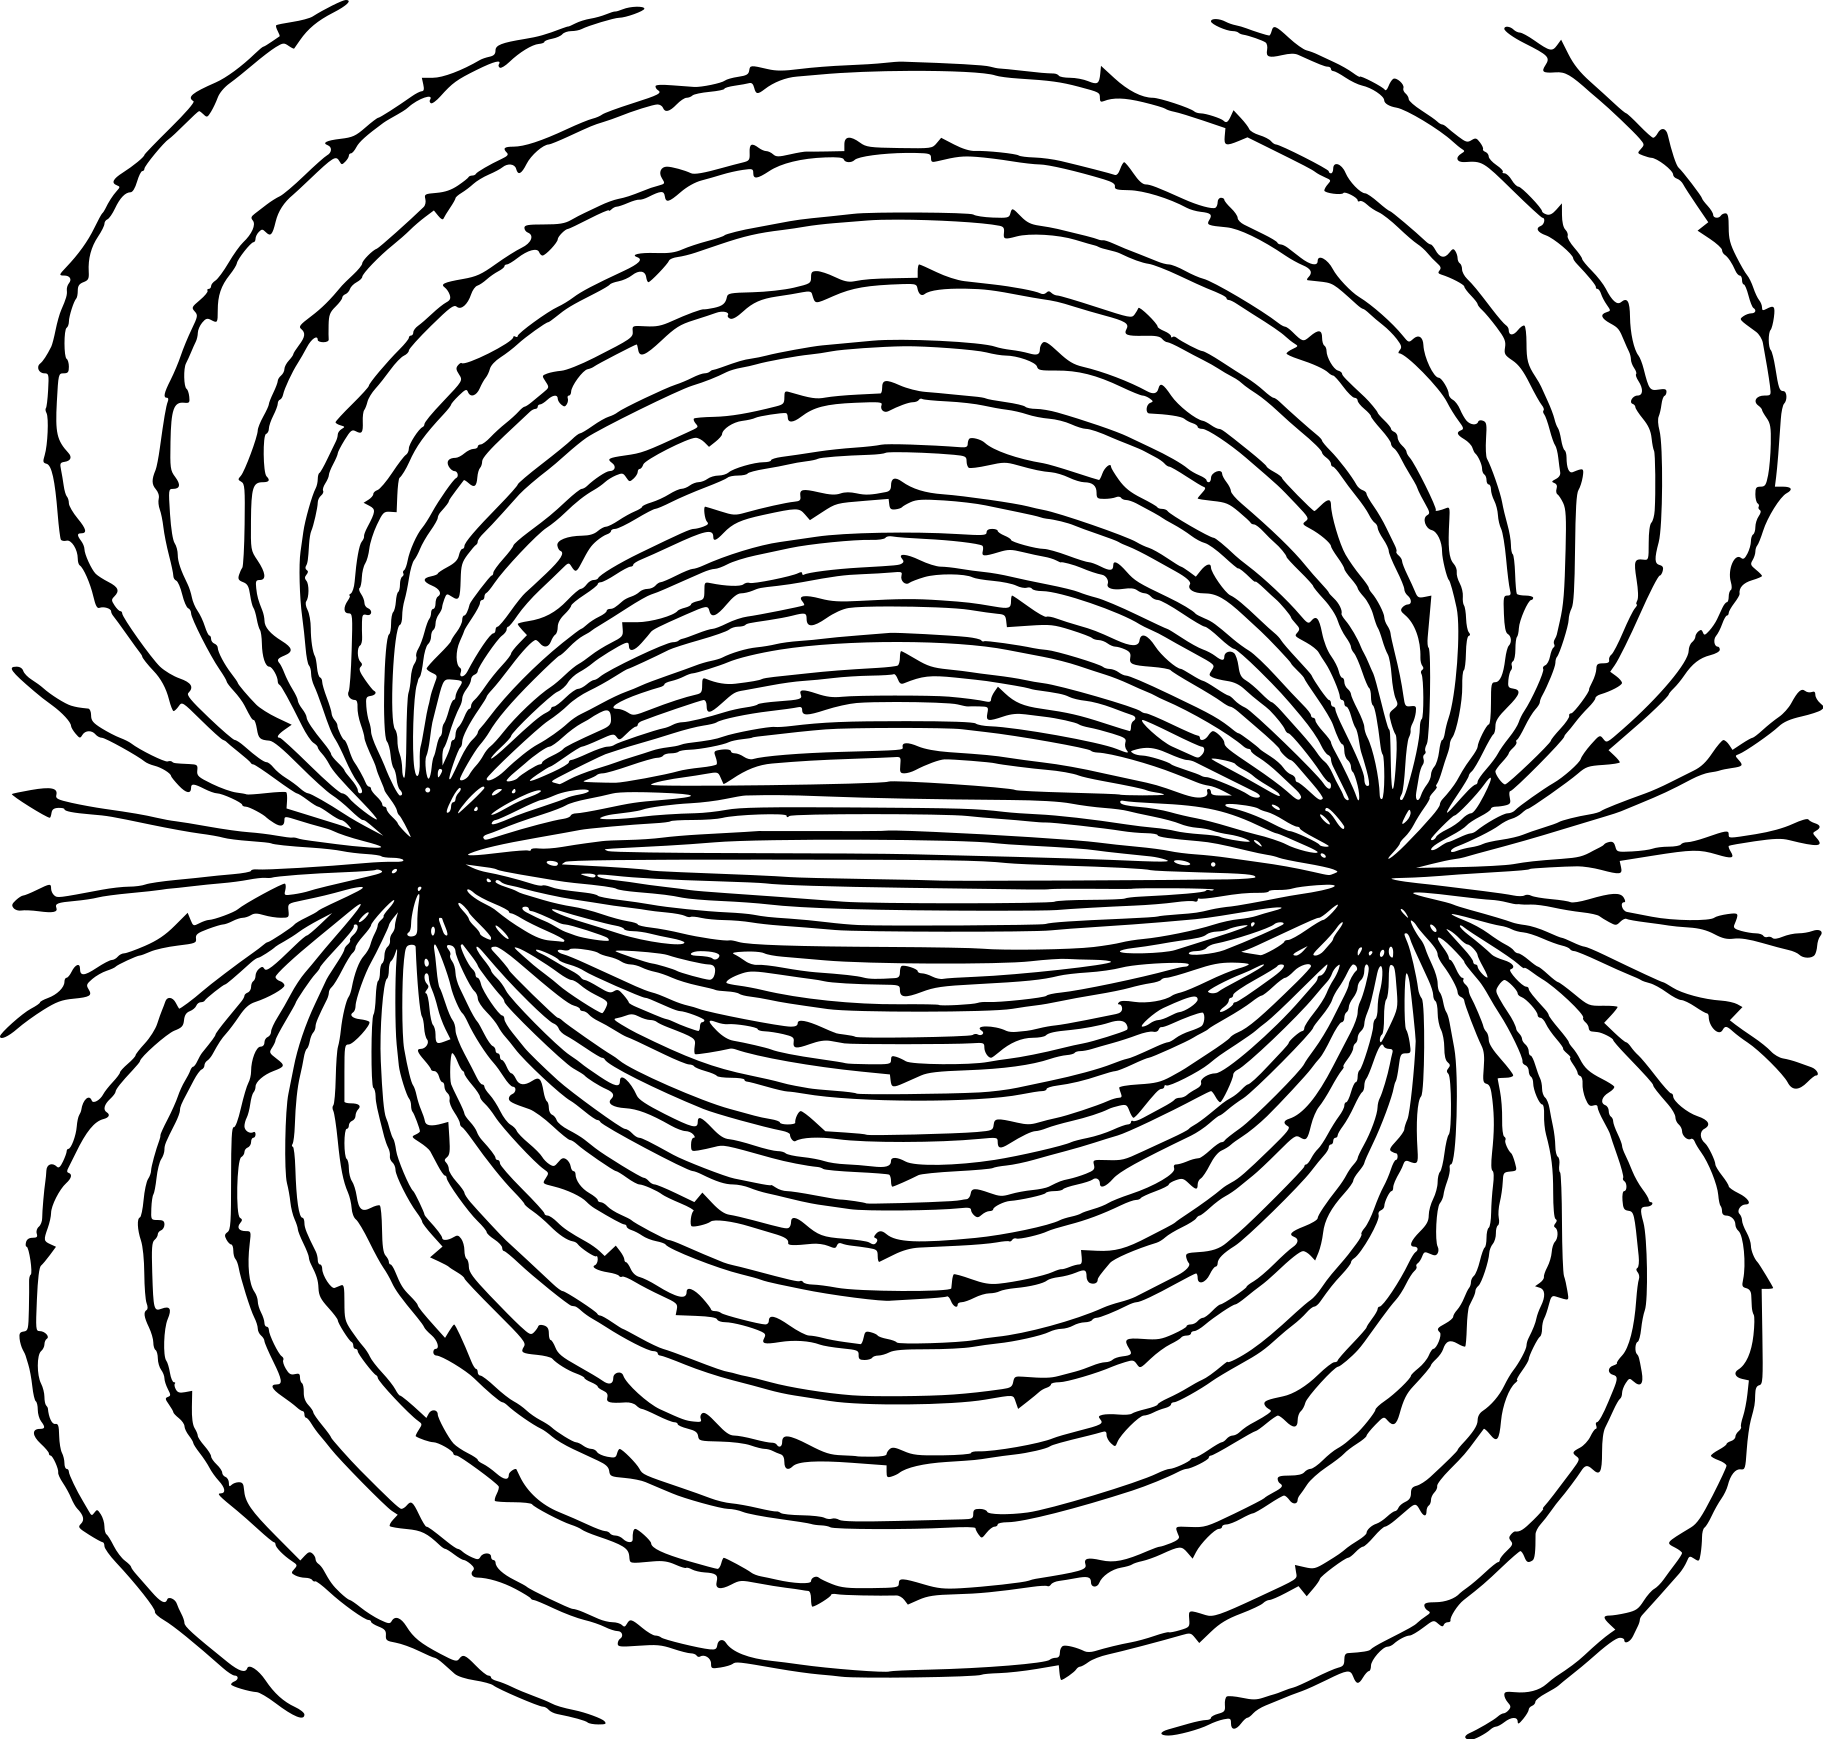
\includegraphics[width = 0.4\tw]{field}
\caption{Поле постоянного магнита}
\end{figure}


\section{Теория}

\subsection{Уравнение движения}  

\begin{equation}
\mathfrak{I} \cdot \vec{\varepsilon} = \vec{M},
\end{equation}
где $\mathfrak{I}$~--- момент инерции стрелки относительно центра масс, $\varepsilon$~--- её угловое ускорение, $M$~--- момент действующих на неё внешних сил:
\begin{equation}
\vec{M} = \left[ \vec{p}_m, \vec{B} \right],
\end{equation}
где $\vec{p}_m$~--- магнитный момент стрелки, $\vec{B}$~--- вектор магнитной индукции внешнего поля.

При малых углах отклонения $\varphi$ стрелки от положения равновесия момент, вызванный горизонтальной компонентой магнитного поля Земли, есть
\begin{equation}
M = - p_m \cdot B \cdot \sin \varphi \approx - p_m \cdot B \cdot \varphi;
\end{equation}
взаимодействие с соседней стрелкой (поле $\vec{B}_1$) вносит вклад
\begin{equation}
M_1 = p_m \cdot B_1 \cdot (\varphi_2 - \varphi_1).
\end{equation}

Так как стрелки одинаковы, $p_m$ и $\mathfrak{I}$ для них будем считать равными. Запишем уравнения движения обеих стрелок:
\begin{equation}
\begin{cases}
\mathfrak{I} \ddot{\varphi}_1 + p_m B \varphi_1 - p_m B_1 (\varphi_2 - \varphi_1) = 0, \\
\mathfrak{I} \ddot{\varphi}_2 + p_m B \varphi_2 - p_m B_1 (\varphi_1 - \varphi_2) = 0
\end{cases}
\quad \Rightarrow \quad
\begin{cases}
\ddot{\alpha}_1 + \omega_1 \alpha_1 = 0; \\
\ddot{\alpha}_2 + \omega_2 \alpha_2 = 0,
\end{cases}
\end{equation}

где после сложения и вычитания уравнений исходной системы введены замены
$$ \alpha_1 \equiv \varphi_1 + \varphi_2, \quad
\alpha_2 \equiv \varphi_1 - \varphi_2, \quad
\omega_1 \equiv \sqrt{\dfrac{p_m B}{\mathfrak{I}}}, \quad
\omega_2 \equiv \sqrt{\dfrac{p_m(B+2B_1)}{\mathfrak{I}}}. $$

Таким образом, колебания складываются из двух (независимых) нормальных мод $\omega_1$ и $\omega_2$, причём синфазные колебания соответствуют моде $\omega_1$, противофазные~--- моде $\omega_2$.

В общем случае происходят сложные колебания каждой из стрелок, природа которых объясняется наличием связи. Если считать, что $B_1 \ll B$ \emph{(связь слабая, стрелки существенно удалены друг от друга),} можно найти связь между $\omega_1$ и $\omega_2$:
\begin{equation}
\omega_2 = \sqrt{\dfrac{p_m(B+2B_1)}{\mathfrak{I}}} = \sqrt{\dfrac{p_m B}{\mathfrak{I}}} \cdot \sqrt{1+\dfrac{2B_1}{B}} \approx \omega_1 \left( 1+\dfrac{B_1}{B} \right).
\end{equation}

Если разность между $\omega_1$ и $\omega_2$ невелика по сравнению с самими величинами, мы видим периодическое увеличение и уменьшение амплитуды колебаний маятников~--- биения;
\begin{equation}
\omega_b = \omega_2 - \omega_1 \approx \dfrac{B_1}{B} \sqrt{\dfrac{p_m B}{\mathfrak{I}}}.
\end{equation}

С учётом $B_1 \simeq \dfrac{\mu_0 p_m}{r^3}$ получаем в приближении слабой связи $\omega_b \propto r^{-3}$.

\subsection{Сильная связь}

Магнитные стрелки предствляют собой магнитные диполи:
\begin{equation}
\vec{B} = \dfrac{\mu_0}{4 \pi} \left(\dfrac{3(\vec{p_m} \cdot\vec{r}) \cdot \vec{r}}{r^5} - \dfrac{\vec p_m}{r^3}\right).
\end{equation}

Поскольку задача плоская, введём такие координаты, что $\vec p_m (0, 0, p_m), \; \vec r (x, 0, z-z')$, и разобьём стрелку на элементарные диполи: $dp_m = p_m \, dz'/l,$ где $l$~--- длина стрелки.

\begin{equation}
d \vec{B} = \dfrac{\mu_0}{4 \pi}
	\left(
		\dfrac{3 \cdot
			\left(dp_m \cdot (z-z') \right)
			\cdot
			\left( \vec{i} \cdot x + \vec{k} \cdot (z-z') \right)
		}{r^5}
	- \dfrac{\vec{k} \cdot dp_m}{r^3}
	\right).
\end{equation}

Выделим компоненты $dB_x$ и $dB_z$ и проинтегрируем их:
%B_x
\begin{equation*}
\begin{split}
B_x &= \dfrac{\mu_0}{4 \pi} \dfrac{p_m}{l} \bigintsss\limits_{-l/2}^{+l/2}
		\dfrac{3 \cdot (z-z') \cdot x \cdot dz'}
		{\left(x^2 + (z-z')^2 \right)^{\frac{5}{2}}}
	= \dfrac{\mu_0}{4 \pi}
	\dfrac{x \cdot p_m}{l}
	\left(
		\frac{1}{\left(x^2 + \left(z-\frac{l}{2}\right)^2 \right)^{\frac{3}{2}}} -
		\frac{1}{\left(x^2 + \left(z+\frac{l}{2}\right)^2 \right)^{\frac{3}{2}}}
	\right);
\\
B_z &= \dfrac{\mu_0}{4 \pi} \dfrac{p_m}{l}
\left( \;
	\bigintsss\limits_{-l/2}^{+l/2}
	\dfrac{3 \cdot (z-z')^2 \cdot dz'}
	{\left(x^2 + (z-z')^2 \right)^{\frac{5}{2}}} -
	 \bigintsss\limits_{-l/2}^{+l/2}
	\dfrac{dz'}
	{\left(x^2 + (z-z')^2 \right)^{\frac{3}{2}}}
\right) = \dfrac{\mu_0}{4 \pi} \dfrac{p_m}{lx^2}
	\dfrac{\left(z+\frac{l}{2}\right)^3}
	{\left(\left(z+\frac{l}{2}\right)^2 + x^2 \right)^{\frac{3}{2}}}.
\end{split}
\end{equation*}

Для второй стрелки с учетом малости углов отклонения элементарный дипольный момент можно положить равным $dp_m = p_m \,dz/l$, тогда
\begin{equation}
d \vec{M} = \left[ d \vec{p}_m, \vec{B} \right] = \vec{k} \, (dp_{mx} \cdot B_z - dp_{mz} \cdot B_x).
\end{equation}
Выражения в скобках упрощаются: $ dp_{mx} \cdot B_z \approx \dfrac{p_m \cdot \varphi}{l} \cdot B_z \,dz, \; dp_{mz} \cdot B_x \approx \dfrac{p_m}{l} \cdot B_x \,dz $;

$$ \int_{-l/2}^{+l/2} B_z \,dz = \dfrac{\mu_0}{2\pi} \dfrac{p_m}{x^2}, \quad
\int_{-l/2}^{+l/2} B_x \,dz = 0 \quad \Rightarrow \quad
M \approx \dfrac{\mu_0}{2\pi} \dfrac{p_m^2}{lx^2} \,\varphi. $$

Следовательно, при наличии сильной связи $\omega_b \propto \sqrt{M} \propto r^{-1}$.


\clearpage
\section{Эксперимент}
Будем размещать стрелки на различных расстояниях $r$ друг от друга и отклонять одну из стрелок из положения равновесия, удерживая другую. Пронаблюдаем $n$ биений и измерим их продолжительность $t = nT_b = 2\pi n/\omega_b$.

\begin{table}[H]
\centering
\resizebox{\lw}{!}{
\begin{tabular}{|c|c|c|c|c|c|c|c|c|c|c|c|c|c|c|}
\hline
$r, \, \cm$     & 17.5  & 19    & 20    & 22    & 23    & 24.5  & 25    & 26    & 27    & 28    & 30    & 32   & 33   & 35    \\ \hline
$t, \, \s$     & 14.35 & 12.37 & 13.23 & 14.41 & 11.28 & 16.07 & 16.72 & 13.26 & 14.13 & 15.92 & 13.68 & 7.65 & 17.4 & 20.25 \\ \hline
$n$     & 5     & 4     & 4     & 4     & 3     & 4     & 4     & 3     & 3     & 3     & 2     & 1    & 2    & 2     \\ \hline
$T_b, \s$     & 2.87  & 3.09  & 3.31  & 3.60  & 3.76  & 4.02  & 4.18  & 4.42  & 4.71  & 5.31  & 6.84  & 7.65 & 8.7  & 10.13 \\ \hline
$\ln r$ & 2.86  & 2.94  & 3.00  & 3.09  & 3.14  & 3.20  & 3.22  & 3.26  & 3.30  & 3.33  & 3.40  & 3.47 & 3.50 & 3.56  \\ \hline
$\ln T$ & 1.05  & 1.13  & 1.20  & 1.28  & 1.32  & 1.39  & 1.43  & 1.49  & 1.55  & 1.67  & 1.92  & 2.03 & 2.16 & 2.32  \\ \hline
\end{tabular}
}
\caption{Данные эксперимента}
\end{table}

Построим график $\ln T(\ln r)$, угловым коэффициентом которого является показатель степени $\alpha$ зависимости $T \propto r^\alpha$.

\begin{figure}[H]
\centering
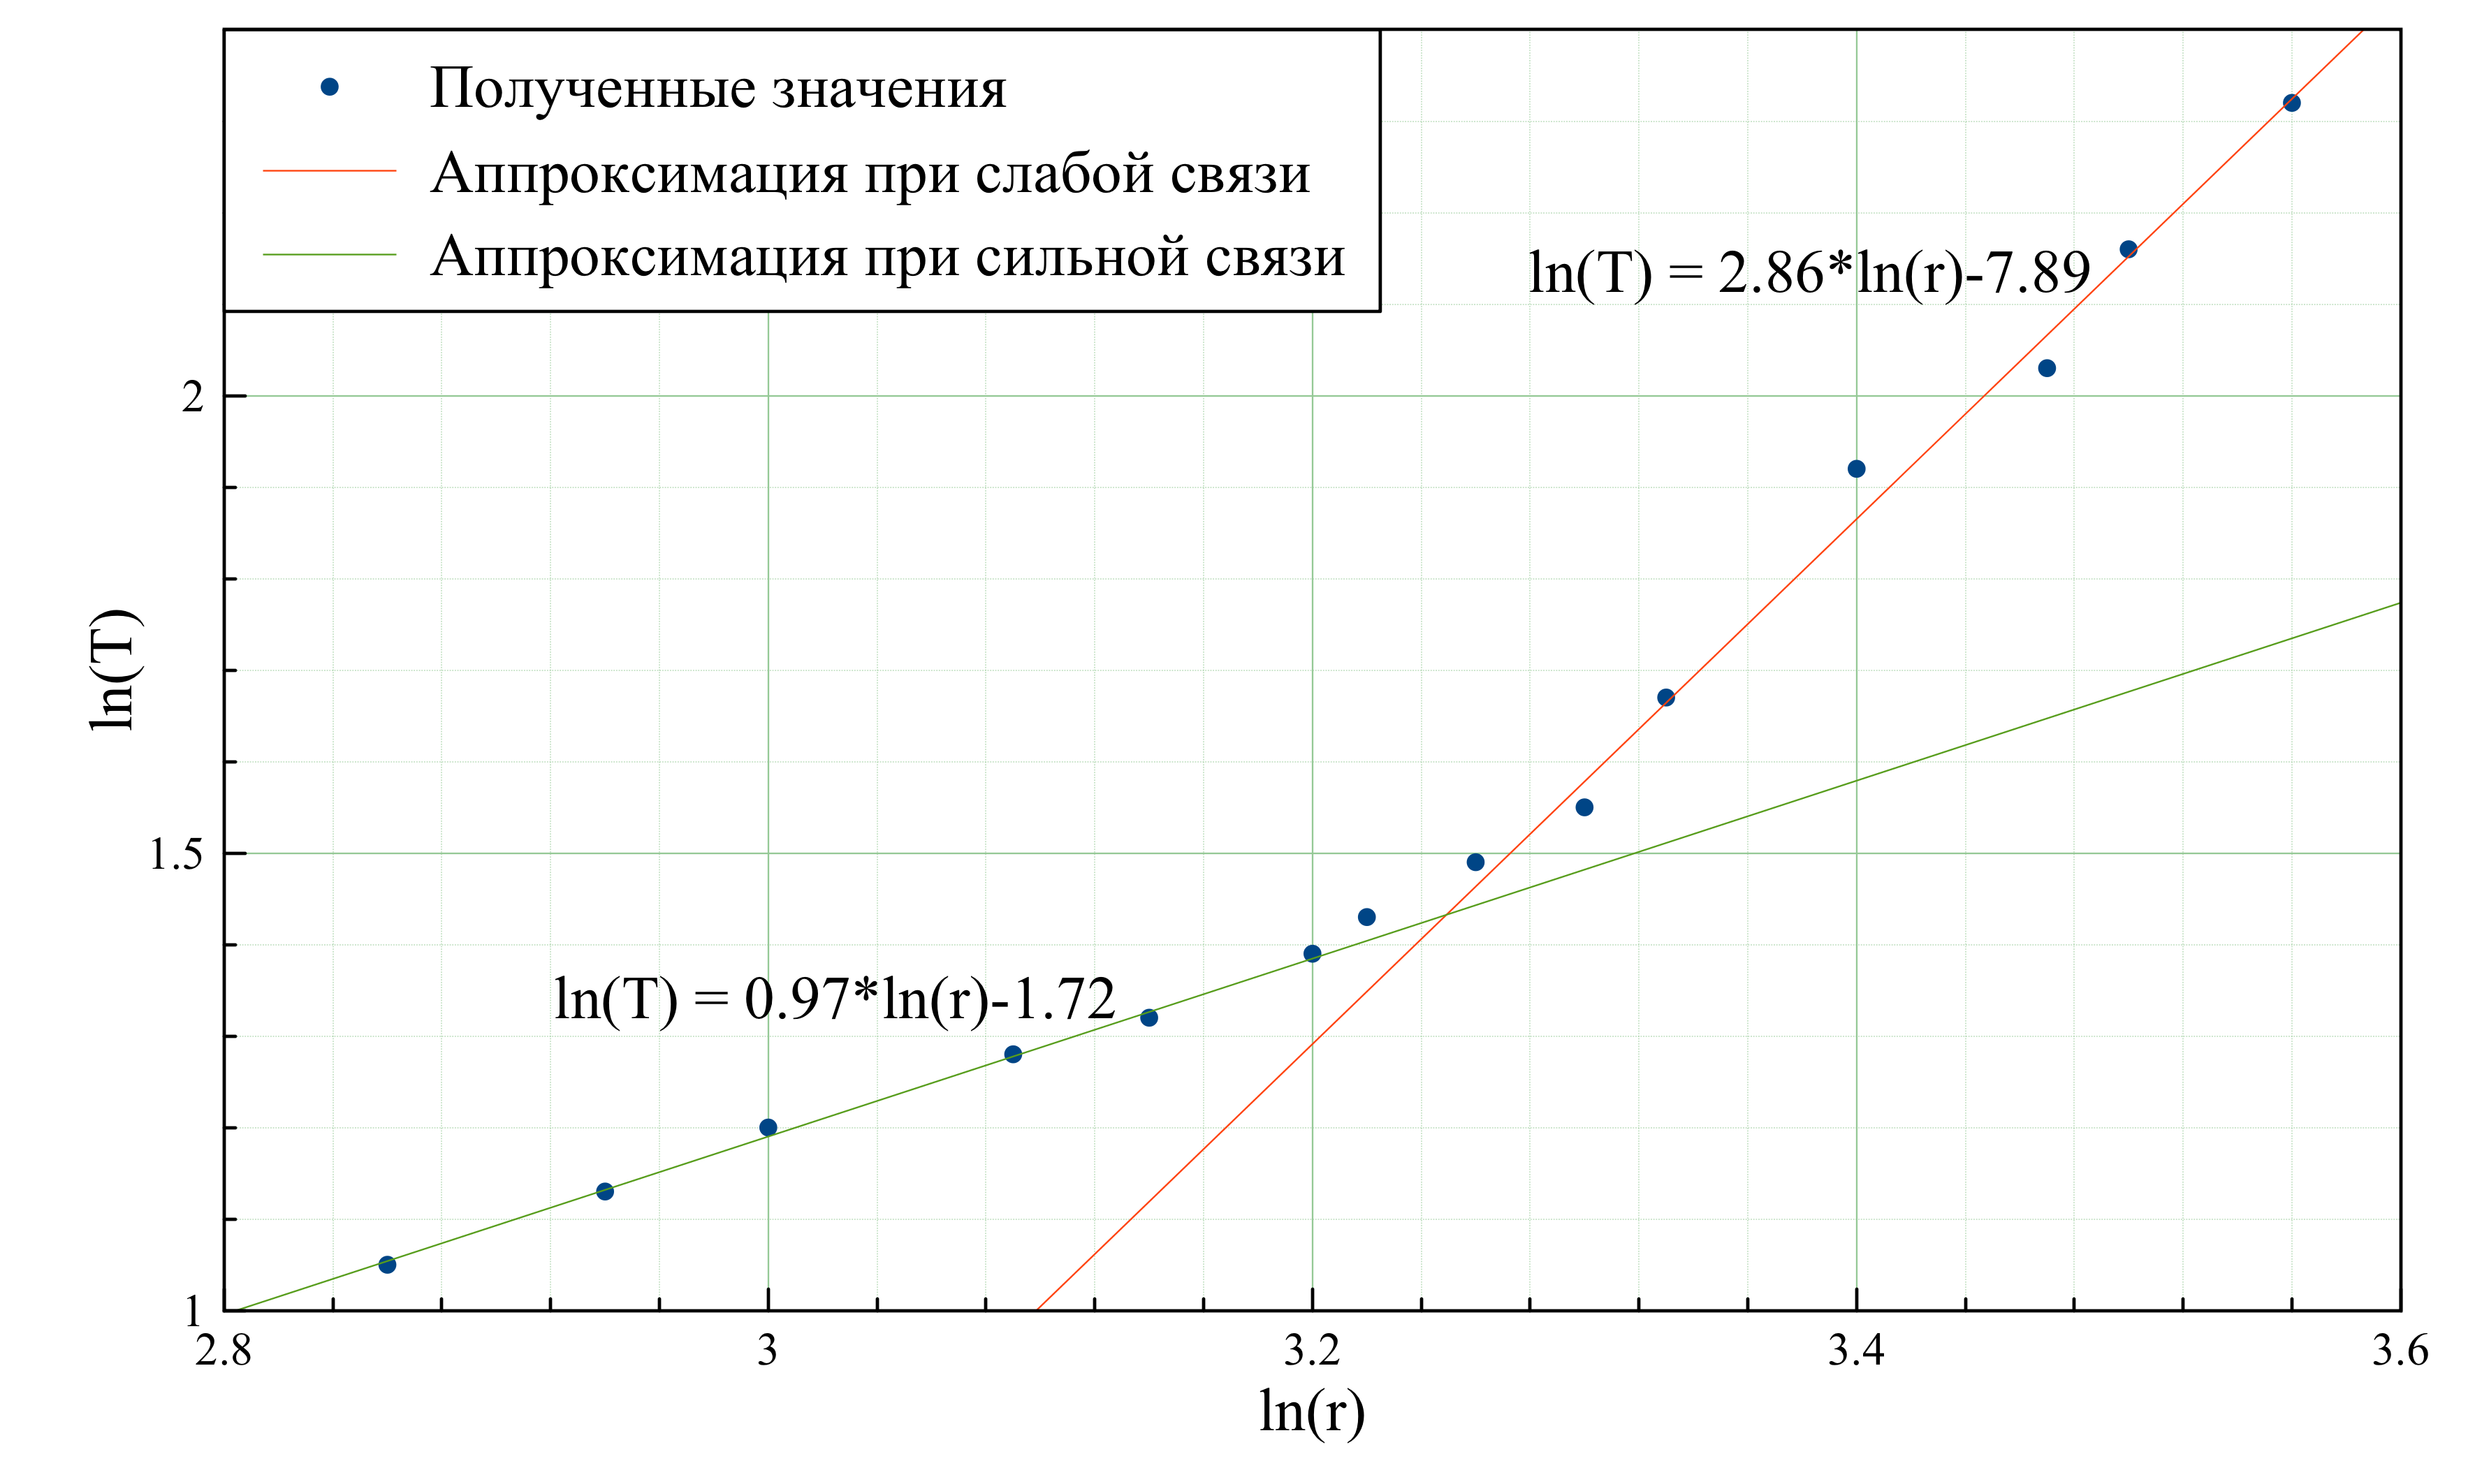
\includegraphics[width = 0.8 \tw]{Logarithmic}
\caption{График в двойном логарифмическом масштабе}
\end{figure}


\section{Выводы}
\begin{itemize}
\item При малых расстояниях между магнитными стрелками их можно рассматривать как связанные маятники с сильной связью и наблюдать явление биений, причём $\omega_b \propto 1/r$.

\item На больших расстояниях влияние поля стрелок уменьшается; $\omega_b \propto 1/r^3$.
\end{itemize}

\end{document}